\section{Realizacja projektu}
Wstęp
  \subsection{Backend}
    \subsubsection{Funkcjonalności wydarzenia}
    \subsubsection{Autoryzacja użytkownika}
    \subsubsection{Komunikacja aplikacji z użytkownikiem}
  \subsection{Frontend}
    \subsubsection{Widoki}
      \begin{itemize}
        \item responsywnść, czli o gridach
        \item html 5, a co jak nie działą :P?
      \end{itemize}
    \subsubsection{Skrypty JS}
      \begin{itemize}
        \item przykłady skryptów z opisami
        \item kompilowalność skryptów
        \item google map
        \item google adres
      \end{itemize}
    \subsubsection{Przykładowe CSS}
      Style CSS \emph{(Cascade Stylesheets)} stanowią o całej szacie graficznej aplikacji. Od nich zależy jak wygląda strona. Określają kolory, rozmiar czcionek, wielkości poszczególnych elementów czy nawet proste animacje. Bez tego strona wyglądałaby nieatrakcyjnie dla użytkowników i straciłaby na funkcjonalności.
      \begin{itemize}
        \item Flexbox\\
          To nowe rozwiązanie pozwalające uzyskać płynny layout\footnote{Dopasowyjący się do rozmiaru okna wygląd strony.}. Pomaga również wyśrodkować w pionie jeden element HTML względem drugiego. Dotychczas twórcy witryn internetowych musieli stosować różnego rodzaju sztuczki, żeby to osiągnać. Na dzień dziejszy\footnote{Dane z dnia 14.12.2014} flexbox jest wspierany przez większość czołowych przeglądarek\footnote{\url{http://caniuse.com/\#search=flexbox}}.
          Z tej technologii korzystaliśmy głównie do wyśrodkowania poszczególnych elementów wzgladem innych.

\begin{code}
	\lstinputlisting[linerange={14-18}, firstnumber=1]{../meetspace/app/assets/stylesheets/_variables.css.scss}
\end{code}\\

Fragment kodu powyżej to przykład oferowanej funkcjonalności preprocesora Sass. \emph{Mixin} to funkcja, która może być wielokrotnie wykorzystana na wielu selektorach CSS.

\begin{code}
	\lstinputlisting[linerange={38-40, 75-75}, firstnumber=1]{../meetspace/app/assets/stylesheets/welcome.css.scss}
\end{code}\\

\emph{@include flex(left)} rozszerzy klasę \emph{search} o właściwości wymienione w pierwszym fragmencie kodu.

Rezultat zastosowania mechanizmu flexbox:\\
\begin{figure}[h]
	\centering
  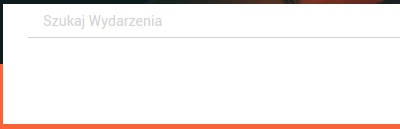
\includegraphics[scale=0.8]{images/flex_before.png}
  \caption{Bez flexbox.}
\end{figure}

\begin{figure}[h]
	\centering
  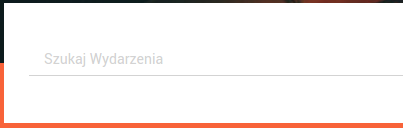
\includegraphics[scale=0.8]{images/flex_after.png}
  \caption{Z wykorzystaniem flexbox.}
\end{figure}


        \item Placeholder\\
          Placeholder to napis wyświetlany w ramce do wpisywania tekstu przez użytkownika. Służy do informowania o roli danego pola. Domyślnym kolorem czcionki jest szary ale nam zależało, żeby cały wygląd współgrał ze sobą. Dlatego chcieliśmy aby kolor placeholder'a był nieco jaśniejszy. Niestety nie da się tego osiągnąć nadając tagowi input  klasę z ustawionym kolorem. Jedyny sposób to wykorzystanie predefiniowanego selektora, odpowiedzialnego za wygląd placeholder'a.

          \begin{code}
            \lstinputlisting[linerange={95-108}, firstnumber=1]{../meetspace/app/assets/stylesheets/layout.css.scss}
          \end{code}\\

          Wartość \emph{\$placeholder} to zmienna Sass przechowująca kolor. Dzięki jej zastosowaniu, w przypadku gdybyśmy chcieli zmienić wartość koloru na inną, nie będziemy musieli tego robić w kilku miejscach, tylko w jednym.

        \item Zapytania medialne \emph{(Media Queries)}\\
          W trakcie tworzenia witryny, która ma dopasowywać się do wielkości ekranu urządzenia, kluczową rolę odgrywają zapytania medialne. W trakcie ładowania pliku css, sprawdzają wielkość, rodzaj ekranu i stosują style zadeklarowane dla określonych rozdzielczości. Dzięki temu można określić na przykład, aby dla urządzeń o szerokości ekranu większej niż 600 pixeli tło strony było inne niż dla węższych ekranów.
          Poniżej został przedstawiony przykład z zapytaniami medialnymi dla
          urządzeń o maksymalnej szerokości 767 pixeli.
          \begin{code}
            \lstinputlisting[linerange={3}]{../meetspace/app/assets/stylesheets/media_queries.css.scss}
          \end{code}\\

      \end{itemize}
  \subsection{Bezpieczeństwo}
    \begin{itemize}
      \item current\_user
      \item boot
      \item autoryzacja api
      \item walidacje
      \item SQL injection
      \item XSS
    \end{itemize}

